\chapter{Méthodologie et environnement de travail}

\section*{Introduction}
\addcontentsline{toc}{section}{Introduction}
Ce chapitre décrit les choix méthodologiques et techniques du projet : pourquoi Scrum, comment le Product Backlog est structuré, quels outils et quelle architecture ont été retenus.

% =============================================================
\section{Choix de la méthode de gestion de projet}
% =============================================================

\subsection{Les méthodes de gestion de projet}
Deux grandes familles de méthodes s'offrent pour la gestion d'un tel projet : Agile et Traditionnelle.

\definecolor{headerbg}{HTML}{d5f5e3}
\setlength{\arrayrulewidth}{1pt}
\begin{longtable}{|>{\raggedright\arraybackslash}p{3cm}|>{\raggedright\arraybackslash}p{5.5cm}|>{\raggedright\arraybackslash}p{6.5cm}|}
\hline
\rowcolor{headerbg}
\textbf{Méthode} & \textbf{Avantages} & \textbf{Inconvénients} \\
\hline
\endfirsthead
\endfoot

\textbf{Agile}
&
\begin{itemize}[left=0pt, topsep=0pt, itemsep=0pt, parsep=0pt, partopsep=0pt]
    \item[$\bullet$] Flexibilité
    \item[$\bullet$] Livraisons fréquentes
    \item[$\bullet$] Collaboration renforcée
    \item[$\bullet$] Amélioration continue
    \item[$\bullet$] Réduction des risques
\end{itemize}
&
\begin{itemize}[left=0pt, topsep=0pt, itemsep=0pt, parsep=0pt, partopsep=0pt]
    \item[$\bullet$] Moins de prévisibilité
    \item[$\bullet$] Documentation limitée
    \item[$\bullet$] Dépendance à l'implication du client
    \item[$\bullet$] Risque de dérive du périmètre
\end{itemize}
\\
\hline

\textbf{Traditionnelle}
&
\begin{itemize}[left=0pt, topsep=0pt, itemsep=0pt, parsep=0pt, partopsep=0pt]
    \item[$\bullet$] Planification détaillée
    \item[$\bullet$] Budget et délais définis
    \item[$\bullet$] Documentation exhaustive
    \item[$\bullet$] Structure hiérarchique claire
\end{itemize}
&
\begin{itemize}[left=0pt, topsep=0pt, itemsep=0pt, parsep=0pt, partopsep=0pt]
    \item[$\bullet$] Rigidité
    \item[$\bullet$] Livraison tardive
    \item[$\bullet$] Moins d'implication du client
    \item[$\bullet$] Risque d'effet tunnel
\end{itemize}
\\
\hline

\caption{Comparaison entre méthode traditionnelle et méthode Agile}
\end{longtable}
\setlength{\arrayrulewidth}{0.4pt}

\subsection*{Pourquoi Scrum ?}
Nous avons choisi Scrum car :
\begin{itemize}
    \item[$\bullet$] Les besoins de PGH ont évolué en cours de projet (règles de paiement, validation des livraisons), rendant toute planification rigide inadaptée.
    \item[$\bullet$] Le système est multi-composants (web Angular, mobile Flutter, back-end Spring Boot, IA FastAPI) avec des dépendances fortes entre modules.
    \item[$\bullet$] Les 4 mois de développement imposaient des livraisons fréquentes et validées à chaque itération par GREPSYS et PGH.
\end{itemize}

% =============================================================
\subsection{Méthodologie SCRUM}
% =============================================================

Le développement s'est organisé autour du cycle de vie Scrum, rythmé par des sprints de deux semaines produisant à chaque itération un incrément fonctionnel livrable. \cite{scrum_guide}

\begin{figure}[H]
\centering
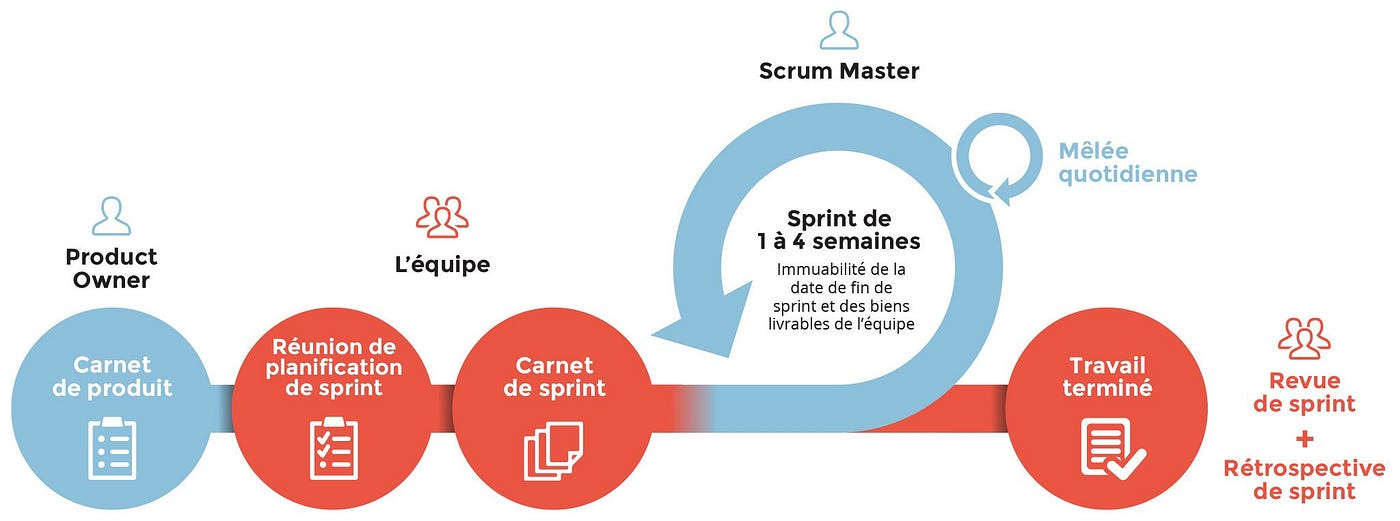
\includegraphics[width=0.65\linewidth]{img/logo/logo_scrum}
\caption{Le cycle de vie Scrum}
\label{fig:scrum-cycle}
\end{figure}

\paragraph*{Rôles Scrum}

\setlength{\arrayrulewidth}{1pt}
\begin{table}[H]
\centering
\begin{tabular}{|p{4cm}|p{11cm}|}
\hline
\rowcolor{headerbg}
\textbf{Rôle} & \textbf{Personne(s)} \\
\hline
Product Owner & M. Marouen Bouallegui \\
\hline
Scrum Master & Mme Lamia Mansouri\\
\hline
Équipe de développement & Mohamed Malek Ben Jemaa et Islem Gharsallah \\
\hline
\end{tabular}
\caption{Répartition des rôles Scrum}
\end{table}
\setlength{\arrayrulewidth}{0.4pt}

% =============================================================
\subsection{Product Backlog}
% =============================================================

Le Product Backlog suivant présente l'ensemble des user stories du projet, organisées en cinq sprints thématiques et priorisées sur une échelle de 1 à 3 (1 étant la priorité maximale).

\definecolor{headerbg}{HTML}{d5f5e3}
\definecolor{sprints}{HTML}{b8e6c8}
\renewcommand{\arraystretch}{0.88}
\setlength{\arrayrulewidth}{1pt}
\begin{longtable}{|c|>{\raggedright\arraybackslash}p{13cm}|c|}
\hline

\rowcolor{headerbg}
\textbf{ID} & \textbf{User Story} & \textbf{Priorité} \\
\hline
\endfirsthead

\rowcolor{headerbg}
\textbf{ID} & \textbf{User Story (suite)} & \textbf{Priorité} \\
\hline
\endhead

\multicolumn{3}{|>{\columncolor{sprints}}c|}{\textbf{Sprint 1 --- Fondation \& Gestion des Ressources} (S1--S2 $\mid$ 25 US)} \\\hline

US-001 & En tant qu'utilisateur, je veux me connecter avec mes identifiants habituels afin d'accéder aux fonctionnalités Fleet~AI correspondant à mon rôle. & 1 \\\hline
US-002 & En tant qu'Administrateur, je veux que les droits de chaque utilisateur soient contrôlés à chaque accès afin que chacun n'utilise que les fonctionnalités autorisées par son rôle. & 1 \\\hline
US-003 & En tant qu'Administrateur, je veux gérer les comptes utilisateurs afin de contrôler les accès au système. & 1 \\\hline
US-004 & En tant qu'Administrateur, je veux assigner un rôle à chaque utilisateur afin de définir ses permissions. & 1 \\\hline
US-005 & En tant qu'Administrateur, je veux gérer les zones géographiques de livraison afin de structurer les opérations par région. & 1 \\\hline
US-006 & En tant qu'Administrateur, je veux consulter le journal d'audit du système afin de tracer toutes les actions critiques. & 1 \\\hline
US-007 & En tant qu'Administrateur, je veux déclencher des sauvegardes des données afin de protéger les informations du système. & 2 \\\hline
US-008 & En tant qu'Administrateur, je veux consulter le tableau de bord avec les statistiques générales afin de superviser l'état du système. & 1 \\\hline
US-009 & En tant que Planificateur, je veux consulter la liste des véhicules avec leur statut afin de connaître les ressources disponibles. & 1 \\\hline
US-010 & En tant qu'Administrateur, je veux gérer les véhicules afin de maintenir le référentiel à jour. & 1 \\\hline
US-011 & En tant que Planificateur, je veux marquer un véhicule en maintenance afin de le retirer temporairement de la planification. & 2 \\\hline
US-012 & En tant que Manager, je veux consulter le taux d'utilisation des véhicules afin d'optimiser la flotte. & 2 \\\hline
US-013 & En tant que Manager, je veux consulter les coûts par véhicule afin de suivre les dépenses opérationnelles. & 2 \\\hline
US-014 & En tant que Planificateur, je veux consulter la disponibilité des chauffeurs afin de planifier les affectations. & 1 \\\hline
US-015 & En tant que Planificateur, je veux consulter les performances des chauffeurs afin de guider les affectations. & 2 \\\hline
US-016 & En tant que Manager, je veux consulter le classement des chauffeurs afin d'identifier les plus et les moins performants. & 2 \\\hline
US-017 & En tant qu'Administrateur, je veux configurer les indicateurs de performance des chauffeurs afin d'adapter le calcul du score global. & 2 \\\hline
US-018 & En tant que Chauffeur, je veux me connecter à l'application mobile afin d'accéder à mes fonctionnalités Fleet~AI. & 1 \\\hline
US-019 & En tant que Chauffeur, je veux consulter mes indicateurs de performance depuis l'application mobile afin de suivre mon activité. & 2 \\\hline
US-020 & En tant que Chauffeur, je veux déclarer ma disponibilité depuis l'application mobile afin de signaler mes périodes de présence. & 1 \\\hline

US-085 & En tant qu'utilisateur, je veux recevoir des notifications en temps réel afin d'être informé des événements importants. & 1 \\\hline
US-086 & En tant qu'utilisateur, je veux recevoir des notifications par email afin de suivre les événements même hors connexion. & 1 \\\hline
US-087 & En tant qu'utilisateur, je veux configurer mes préférences de notification afin de recevoir uniquement les alertes pertinentes. & 2 \\\hline
US-088 & En tant qu'utilisateur, je veux voir l'historique de mes notifications afin de retrouver les informations reçues. & 2 \\\hline
US-138 & En tant que Chauffeur, je veux configurer mes préférences de notification sur l'application mobile afin de gérer mes alertes. & 2 \\\hline
\multicolumn{3}{|>{\columncolor{sprints}}c|}{\textbf{Sprint 2 --- Gestion des Clients \& Commandes} (S3--S4 $\mid$ 30 US)} \\\hline

US-094 & En tant que Responsable des Engagements Clients, je veux gérer le référentiel clients afin de maintenir une base clients à jour. & 1 \\\hline
US-095 & En tant que Responsable des Engagements Clients, je veux gérer les adresses de livraison de mes clients afin d'assurer des livraisons précises à chaque emplacement. & 1 \\\hline
US-096 & En tant que Responsable des Engagements Clients, je veux consulter l'historique complet d'un client afin de piloter la relation client. & 1 \\\hline
US-097 & En tant que Responsable des Engagements Clients, je veux bloquer un client afin de suspendre ses commandes en cas de litige. & 1 \\\hline
US-098 & En tant que Responsable des Engagements Clients, je veux débloquer un client afin de rétablir ses droits après régularisation. & 1 \\\hline
US-099 & En tant que Responsable des Engagements Clients, je veux voir la liste des clients bloqués afin d'en assurer le suivi. & 1 \\\hline
US-100 & En tant que Responsable des Engagements Clients, je veux que la création d'une commande soit refusée pour un client bloqué afin d'éviter toute expédition non autorisée. & 1 \\\hline
US-101 & En tant que Responsable des Engagements Clients, je veux activer ou désactiver des comptes clients afin de gérer leurs accès. & 2 \\\hline
US-102 & En tant que Responsable des Engagements Clients, je veux définir un niveau de service par client afin de garantir le respect des engagements contractuels. & 2 \\\hline
US-103 & En tant que Client, je veux noter le service et le chauffeur après livraison afin de partager mon retour d'expérience. & 2 \\\hline
US-104 & En tant que Client, je veux voir l'estimation d'arrivée de mes livraisons afin de planifier ma réception. & 2 \\\hline
US-007b & En tant que Responsable des Engagements Clients, je veux créer une commande avec vérification de la disponibilité du stock afin d'éviter les ruptures. & 1 \\\hline
US-008b & En tant que Planificateur, je veux que le système suive le cycle de vie complet d'une commande afin d'assurer la traçabilité de bout en bout. & 1 \\\hline
US-009b & En tant que Client, je veux consulter le statut de mes commandes afin de suivre mes livraisons. & 1 \\\hline
US-010b & En tant que Client, je veux annuler une commande avant son expédition afin d'ajuster mes besoins. & 1 \\\hline
US-011b & En tant que Planificateur, je veux voir les commandes en attente d'affectation triées par priorité afin d'organiser le traitement. & 1 \\\hline
US-012b & En tant que Responsable des Engagements Clients, je veux consulter le stock réel disponible afin de gérer les commandes en conséquence. & 1 \\\hline
US-013b & En tant que Client, je veux consulter le stock disponible afin de passer commande en connaissance de cause. & 1 \\\hline
US-014b & En tant que Responsable des Engagements Clients, je veux définir le stock visible par les clients afin de contrôler les informations publiées. & 1 \\\hline
US-015b & En tant que Responsable des Engagements Clients, je veux modifier une commande existante afin de corriger ou d'adapter une demande. & 2 \\\hline
US-016b & En tant que Responsable des Engagements Clients, je veux reprogrammer une livraison à la demande du client afin d'adapter la date à ses contraintes. & 2 \\\hline
US-017b & En tant que Planificateur, je veux filtrer les commandes par statut, date, client et zone afin de gagner en efficacité. & 2 \\\hline
US-018b & En tant que Responsable des Engagements Clients, je veux gérer les priorités des commandes afin d'assurer le traitement des demandes urgentes en premier. & 2 \\\hline
US-019b & En tant que Responsable des Engagements Clients, je veux associer un niveau de priorité au client afin de personnaliser le service rendu. & 2 \\\hline
US-020b & En tant que Client, je veux consulter l'historique de mes livraisons passées afin de suivre mon activité. & 2 \\\hline
US-139 & En tant que Client, je veux noter une livraison depuis l'application mobile afin de partager mon évaluation. & 2 \\\hline

US-089 & En tant que Planificateur, je veux que des notifications soient envoyées à chaque étape du workflow afin d'assurer la coordination entre acteurs. & 1 \\\hline
US-090 & En tant que Client, je veux recevoir une notification à l'approche du chauffeur afin de me préparer à la réception. & 2 \\\hline
US-092 & En tant que Client, je veux recevoir des rappels automatiques avant ma livraison afin de ne pas manquer la réception. & 3 \\\hline
\multicolumn{3}{|>{\columncolor{sprints}}c|}{\textbf{Sprint 3 --- Planification \& Optimisation} (S5--S6 $\mid$ 21 US)} \\\hline

US-021 & En tant que Planificateur, je veux assigner manuellement une commande à un chauffeur et un véhicule afin d'organiser les livraisons. & 1 \\\hline
US-022 & En tant que Planificateur, je veux créer un plan de livraison quotidien regroupant plusieurs commandes afin d'optimiser les tournées. & 1 \\\hline
US-023 & En tant que Planificateur, je veux voir la charge de chaque chauffeur afin d'équilibrer les affectations. & 1 \\\hline
US-024 & En tant que Planificateur, je veux vérifier la capacité du véhicule avant affectation afin d'éviter les surcharges. & 1 \\\hline
US-025 & En tant que Planificateur, je veux réassigner une livraison en cas de problème afin de garantir la continuité du service. & 1 \\\hline
US-026 & En tant que Planificateur, je veux que le système estime les distances entre points de livraison afin d'optimiser les itinéraires. & 1 \\\hline
US-027 & En tant que Planificateur, je veux gérer les créneaux horaires de livraison afin de respecter les engagements clients. & 2 \\\hline
US-028 & En tant que Planificateur, je veux créer des plans hebdomadaires récurrents afin de faciliter la planification répétitive. & 2 \\\hline
US-029 & En tant que Planificateur, je veux générer un document de chargement pour l'entrepôt afin de préparer les expéditions. & 2 \\\hline
US-030 & En tant que Planificateur, je veux reprogrammer les livraisons échouées afin d'assurer leur traitement ultérieur. & 2 \\\hline
US-031 & En tant que Planificateur, je veux définir des règles d'incompatibilité entre chauffeurs et zones afin d'éviter les erreurs d'attribution. & 3 \\\hline
US-037 & En tant que Planificateur, je veux recevoir des suggestions du chauffeur le plus adapté afin d'optimiser les affectations. & 2 \\\hline
US-032 & En tant que Planificateur, je veux recevoir des suggestions d'itinéraires optimisés afin de réduire les distances parcourues. & 1 \\\hline
US-033 & En tant que Planificateur, je veux accepter, modifier ou rejeter chaque suggestion afin de garder le contrôle sur les décisions. & 1 \\\hline
US-034 & En tant que Chauffeur, je veux voir l'itinéraire optimisé sur une carte afin de naviguer efficacement. & 1 \\\hline
US-035 & En tant que Planificateur, je veux que le système respecte les contraintes métier lors de l'optimisation afin de garantir la faisabilité des plans. & 1 \\\hline
US-036 & En tant que Planificateur, je veux que les parties prenantes soient notifiées après validation du plan afin d'assurer la coordination. & 1 \\\hline
US-038 & En tant que Planificateur, je veux envoyer des retours au système afin d'améliorer la qualité des suggestions futures. & 2 \\\hline
US-131 & En tant que Chauffeur, je veux voir mes livraisons et l'itinéraire optimisé sur la carte mobile afin de démarrer ma tournée. & 1 \\\hline
US-106 & En tant que Planificateur, je veux un tableau de bord opérationnel en temps réel afin de suivre l'avancement des livraisons. & 1 \\\hline

US-091 & En tant que Planificateur, je veux recevoir des alertes afin d'être informé des anomalies et risques détectés. & 2 \\\hline
\multicolumn{3}{|>{\columncolor{sprints}}c|}{\textbf{Sprint 4 --- Exécution des Livraisons \& Paiement} (S7--S8 $\mid$ 32 US)} \\\hline

US-039 & En tant que Chauffeur, je veux démarrer une livraison et voir ses détails afin de préparer la remise de commande. & 1 \\\hline
US-040 & En tant que Chauffeur, je veux confirmer la livraison avec la signature du client afin de disposer d'une preuve numérique. & 1 \\\hline
US-041 & En tant que Chauffeur, je veux prendre des photos géolocalisées afin de constituer une preuve de livraison. & 1 \\\hline
US-042 & En tant que Chauffeur, je veux scanner les codes des articles livrés afin de valider la conformité de la commande. & 2 \\\hline
US-043 & En tant que Chauffeur, je veux signaler un problème lors d'une livraison afin d'alerter le planificateur. & 1 \\\hline
US-044 & En tant que Planificateur, je veux suivre en temps réel la position des chauffeurs afin de superviser les tournées. & 1 \\\hline
US-045 & En tant que Planificateur, je veux que le statut de la commande soit mis à jour automatiquement afin de refléter l'avancement réel. & 1 \\\hline
US-046 & En tant que Responsable des Engagements Clients, je veux générer un bordereau de livraison afin de documenter chaque tournée. & 2 \\\hline
US-047 & En tant que Chauffeur, je veux remplir une checklist de départ véhicule afin de vérifier l'état du camion avant la tournée. & 2 \\\hline
US-048 & En tant que Client, je veux suivre ma livraison en temps réel afin de connaître l'heure d'arrivée estimée. & 2 \\\hline
US-049 & En tant que Planificateur, je veux que le système détecte les retards automatiquement afin d'alerter les parties concernées. & 2 \\\hline
US-050 & En tant que Manager, je veux consulter les indicateurs de livraison du jour afin de superviser les opérations. & 2 \\\hline
US-105 & En tant que Manager, je veux un tableau de bord stratégique afin de suivre les indicateurs clés de performance. & 1 \\\hline
US-107 & En tant que Manager, je veux exporter les rapports afin de partager les résultats avec la direction. & 1 \\\hline
US-108 & En tant que Manager, je veux voir les tendances sur plusieurs mois afin d'identifier les évolutions. & 1 \\\hline
US-114 & En tant que Manager, je veux un tableau de bord financier afin de suivre les coûts et revenus liés au transport. & 3 \\\hline
US-063 & En tant que Planificateur, je veux voir le statut de paiement d'une commande afin d'autoriser ou bloquer la livraison. & 1 \\\hline
US-064 & En tant que Chauffeur, je veux enregistrer un paiement par chèque afin de le transmettre au Responsable pour validation. & 1 \\\hline
US-065 & En tant que Responsable des Engagements Clients, je veux enregistrer un paiement à crédit afin de gérer les encours clients. & 1 \\\hline
US-066 & En tant que Chauffeur, je veux consulter le récapitulatif de mes encaissements du jour afin de vérifier ma collecte. & 1 \\\hline
US-067 & En tant que Responsable des Engagements Clients, je veux rapprocher les encaissements avec les commandes livrées afin d'assurer la cohérence comptable. & 1 \\\hline
US-068 & En tant que Responsable des Engagements Clients, je veux gérer les encours clients afin de contrôler les risques financiers. & 2 \\\hline
US-069 & En tant que Manager, je veux voir les statistiques de paiement afin d'analyser les modes de règlement utilisés. & 2 \\\hline
US-070 & En tant que Client, je veux consulter mes factures et paiements afin de suivre mes transactions. & 2 \\\hline
US-071 & En tant que Responsable des Engagements Clients, je veux que les justificatifs de paiement soient conservés afin de répondre aux obligations de traçabilité. & 2 \\\hline
US-072 & En tant que Chauffeur, je veux remettre un justificatif de paiement au client après encaissement afin de documenter la transaction. & 3 \\\hline
US-132 & En tant que Chauffeur, je veux mettre à jour le statut de chaque livraison depuis l'application mobile afin d'informer le planificateur en temps réel. & 1 \\\hline
US-133 & En tant que Chauffeur, je veux capturer la signature du client sur l'application mobile afin de valider la remise de commande. & 1 \\\hline
US-134 & En tant que Chauffeur, je veux prendre des photos géolocalisées depuis l'application mobile afin de constituer une preuve de livraison. & 1 \\\hline
US-135 & En tant que Chauffeur, je veux valider les articles livrés depuis l'application mobile afin de confirmer la conformité de la commande. & 2 \\\hline
US-136 & En tant que Chauffeur, je veux remplir la checklist de départ sur l'application mobile afin d'attester de l'état du véhicule. & 2 \\\hline

\multicolumn{3}{|>{\columncolor{sprints}}c|}{\textbf{Sprint 5 --- Prédiction, Réclamations \& Notifications} (S9--S10 $\mid$ 34 US)} \\\hline

US-073 & En tant que Planificateur, je veux des prédictions de la demande par zone et par jour afin d'anticiper les besoins en ressources. & 1 \\\hline
US-074 & En tant que Planificateur, je veux des prédictions de retard pour chaque tournée afin de prendre des mesures préventives. & 1 \\\hline
US-075 & En tant que Manager, je veux voir le niveau de confiance des prédictions afin d'évaluer leur fiabilité. & 2 \\\hline
US-076 & En tant qu'Administrateur, je veux que les modèles de prédiction soient mis à jour périodiquement afin de maintenir leur précision. & 2 \\\hline
US-077 & En tant que Manager, je veux comparer les prédictions au réel afin d'évaluer la performance du système. & 2 \\\hline
US-078 & En tant que Planificateur, je veux des recommandations pour le dimensionnement de la flotte afin d'optimiser les ressources disponibles. & 3 \\\hline
US-079 & En tant que Client, je veux soumettre une réclamation afin de signaler un problème lié à ma livraison. & 1 \\\hline
US-080 & En tant que Responsable des Engagements Clients, je veux voir la liste des réclamations et les traiter afin d'assurer la satisfaction client. & 1 \\\hline
US-081 & En tant que Client, je veux suivre le statut de ma réclamation afin d'être informé de son traitement. & 1 \\\hline
US-082 & En tant que Manager, je veux des statistiques sur les réclamations afin d'identifier les points d'amélioration. & 2 \\\hline
US-083 & En tant que Responsable des Engagements Clients, je veux que les réclamations non traitées soient escaladées automatiquement afin de respecter les délais de réponse. & 2 \\\hline
US-084 & En tant que Manager, je veux identifier les causes récurrentes des réclamations afin de mettre en place des actions correctives. & 3 \\\hline
US-137 & En tant que Chauffeur, je veux signaler un problème directement depuis l'application mobile afin de l'enregistrer en temps réel. & 1 \\\hline
US-111 & En tant que Manager, je veux personnaliser mon tableau de bord afin d'afficher les indicateurs les plus pertinents pour mon activité. & 2 \\\hline
US-113 & En tant que Manager, je veux un tableau de bord de performance des chauffeurs afin d'évaluer la qualité du service rendu. & 2 \\\hline
US-110 & En tant que Manager, je veux recevoir des rapports récapitulatifs réguliers afin de suivre l'activité sans connexion permanente. & 2 \\\hline
US-115 & En tant qu'Administrateur, je veux superviser les temps de réponse du système afin de garantir une expérience utilisateur fluide. & 1 \\\hline
US-116 & En tant qu'Administrateur, je veux configurer des alertes sur les indicateurs clés afin d'être averti en cas de dépassement de seuil. & 2 \\\hline
US-117 & En tant qu'Administrateur, je veux que les données fréquemment consultées soient optimisées afin de réduire les temps d'attente pour les utilisateurs. & 2 \\\hline
US-118 & En tant qu'Administrateur, je veux que toutes les actions des utilisateurs soient journalisées afin d'assurer la traçabilité et la conformité réglementaire. & 1 \\\hline
US-112 & En tant qu'Administrateur, je veux consulter les métriques d'utilisation du système afin de détecter les anomalies de fonctionnement. & 2 \\\hline
US-140 & En tant que Chauffeur, je veux utiliser l'application en mode hors ligne afin de continuer à travailler sans connexion réseau. & 1 \\\hline
US-141 & En tant que Chauffeur, je veux que mes données se synchronisent automatiquement au retour du réseau afin d'éviter toute perte d'information. & 1 \\\hline
US-142 & En tant que Planificateur, je veux que les conflits de synchronisation soient gérés automatiquement afin d'assurer la cohérence des données. & 2 \\\hline
US-143 & En tant que Chauffeur, je veux voir un indicateur de connexion sur l'application afin de savoir si je suis en mode hors ligne. & 2 \\\hline

\hline
\rowcolor{headerbg}
\multicolumn{2}{|c|}{\textbf{Total}} & \textbf{133 US} \\
\hline

\caption{Product Backlog de Fleet~AI --- 5 sprints, 133 User Stories}
\end{longtable}
\setlength{\arrayrulewidth}{0.4pt}


% =============================================================
\section{Planification de projet}
% =============================================================

Le projet Fleet~AI s'est déroulé sur \textbf{16 semaines} (Février -- Mai~2025), découpées en phases dont la durée reflète la complexité technique de chaque incrément. Le diagramme de Gantt ci-dessous illustre la planification réelle du projet.


% ============================================================
% DIAGRAMME DE GANTT — Fleet AI (Février – Mai 2025)
% Diagramme dessiné en pur TikZ pour garantir l'affichage
% des labels à l'intérieur des barres.
% ============================================================

\definecolor{ganttDark}{RGB}{30,110,50}
\definecolor{ganttMid}{RGB}{30,110,50}
\definecolor{ganttBar}{HTML}{d5f5e3}
\definecolor{ganttBarLight}{HTML}{b7e4c7}
\definecolor{ganttGrey}{HTML}{e0e0e0}
\definecolor{ganttGreyDark}{HTML}{646464}
\definecolor{ganttTextDark}{RGB}{30,110,50}
\definecolor{ganttTextGrey}{HTML}{444444}
\definecolor{ganttBg}{HTML}{ffffff}
\definecolor{ganttRowAlt}{HTML}{f7f7f7}

\begin{figure}[htbp]
\centering
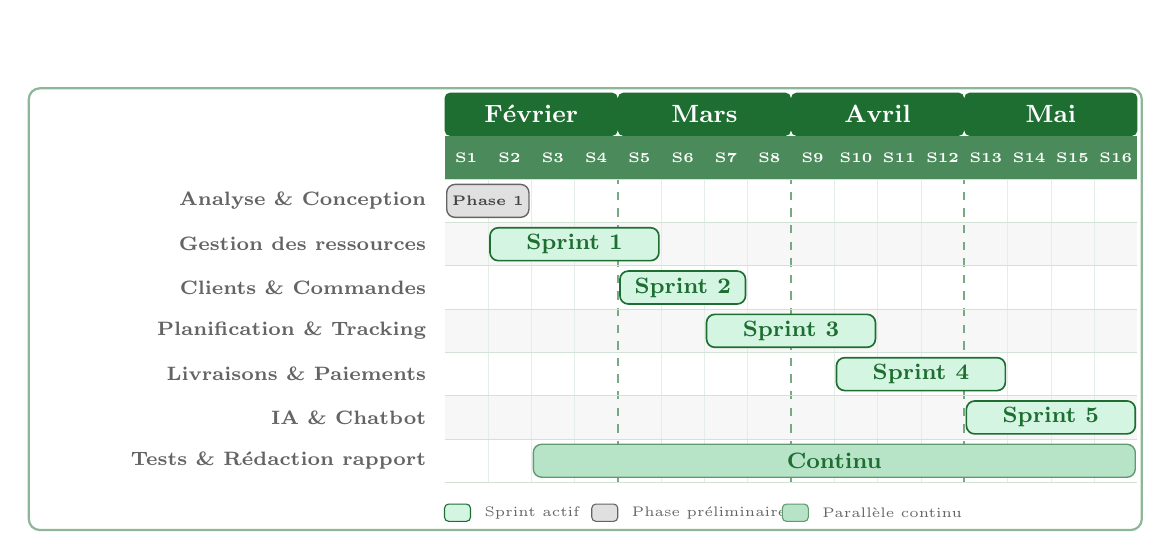
\begin{tikzpicture}[x=0.55cm, y=0.55cm]

  % Dimensions ajustées :
  % Colonne de gauche (titres longs) : de 0 à 5.0
  % Grille des semaines : de 5.1 à 21.1 (16 semaines)

  %% ── Fond général ─────────────────────────────────────────
  \fill[ganttBg, rounded corners=4pt] (-4.5,-0.5) rectangle (21.2,10.5);

  %% ── Fond alterné des lignes ───────────────────────────────
  \foreach \row/\col in {7/ganttBg, 6/ganttRowAlt, 5/ganttBg,
                          4/ganttRowAlt, 3/ganttBg, 2/ganttRowAlt, 1/ganttBg}{
    \fill[\col] (5.1,\row-1) rectangle (21.1,\row);
  }

  %% ── En-tête mois ─────────────────────────────────────────
  \fill[ganttDark,  rounded corners=2pt] (5.1,8)   rectangle (9.1,9);
  \fill[ganttMid,   rounded corners=2pt] (9.1,8)   rectangle (13.1,9);
  \fill[ganttDark,  rounded corners=2pt] (13.1,8)  rectangle (17.1,9);
  \fill[ganttMid,   rounded corners=2pt] (17.1,8)  rectangle (21.1,9);

  \node[text=white, font=\small\bfseries] at (7.1,  8.5) {F\'evrier};
  \node[text=white, font=\small\bfseries] at (11.1, 8.5) {Mars};
  \node[text=white, font=\small\bfseries] at (15.1, 8.5) {Avril};
  \node[text=white, font=\small\bfseries] at (19.1, 8.5) {Mai};

  %% ── En-tête semaines ──────────────────────────────────────
  \fill[ganttDark!80] (5.1,7) rectangle (21.1,8);
  \foreach \i in {1,...,16}{
    \node[text=white, font=\tiny\bfseries]
      at (5.1+\i-0.5, 7.5) {S\i};
  }

  %% ── Grille verticale : séparateurs de mois (tiretés) ─────
  \foreach \x in {9.1, 13.1, 17.1}{
    \draw[ganttMid!60, dashed, line width=0.6pt] (\x,0) -- (\x,7);
  }

  %% ── Grille verticale : semaines (très légère) ────────────
  \foreach \x in {6.1,7.1,8.1, 10.1,11.1,12.1, 14.1,15.1,16.1, 18.1,19.1,20.1}{
    \draw[ganttDark!12, line width=0.2pt] (\x,0) -- (\x,7);
  }

  %% ── Grille horizontale ───────────────────────────────────
  \foreach \y in {0,...,7}{
    \draw[ganttDark!20, line width=0.3pt] (5.1,\y) -- (21.1,\y);
  }

  %% ── Labels de lignes (à gauche) - TITRES DES TÂCHES ────
  \node[anchor=east, font=\scriptsize\bfseries, text=ganttGreyDark, align=right, text width=4.5cm]
    at (4.9, 6.5) {Analyse \& Conception};
  \node[anchor=east, font=\scriptsize\bfseries, text=ganttGreyDark, align=right, text width=4.5cm]
    at (4.9, 5.5) {Gestion des ressources};
  \node[anchor=east, font=\scriptsize\bfseries, text=ganttGreyDark, align=right, text width=4.5cm]
    at (4.9, 4.5) {Clients \& Commandes};
  \node[anchor=east, font=\scriptsize\bfseries, text=ganttGreyDark, align=right, text width=4.5cm]
    at (4.9, 3.5) {Planification \& Tracking};
  \node[anchor=east, font=\scriptsize\bfseries, text=ganttGreyDark, align=right, text width=4.5cm]
    at (4.9, 2.5) {Livraisons \& Paiements};
  \node[anchor=east, font=\scriptsize\bfseries, text=ganttGreyDark, align=right, text width=4.5cm]
    at (4.9, 1.5) {IA \& Chatbot};
  \node[anchor=east, font=\scriptsize\bfseries, text=ganttGreyDark, align=right, text width=4.5cm]
    at (4.9, 0.5) {Tests \& R\'edaction rapport};

  %% ═══════════════════════════════════════════════════════════
  %% BARRES DE TÂCHES - "Sprint X" à l'intérieur
  %% ═══════════════════════════════════════════════════════════

  %% Ligne 7 : Analyse & Conception — S1-S2 (x=5.1, w=2)
  \fill[ganttGrey, draw=ganttGreyDark, rounded corners=3pt, line width=0.5pt]
    (5.15, 6.12) rectangle (7.05, 6.88);
  \node[font=\tiny\bfseries, text=ganttTextGrey, align=center]
    at (6.1, 6.5) {Phase 1};

  %% Ligne 6 : Sprint 1 — S2-S5 (x=6.1, w=4)
  \fill[ganttBar, draw=ganttMid, rounded corners=3pt, line width=0.6pt]
    (6.15, 5.12) rectangle (10.05, 5.88);
  \node[font=\footnotesize\bfseries, text=ganttTextDark, align=center]
    at (8.1, 5.5) {Sprint 1};

  %% Ligne 5 : Sprint 2 — S5-S8 (x=9.1, w=3)
  \fill[ganttBar, draw=ganttMid, rounded corners=3pt, line width=0.6pt]
    (9.15, 4.12) rectangle (12.05, 4.88);
  \node[font=\footnotesize\bfseries, text=ganttTextDark, align=center]
    at (10.6, 4.5) {Sprint 2};

  %% Ligne 4 : Sprint 3 — S7-S10 (x=11.1, w=4)
  \fill[ganttBar, draw=ganttMid, rounded corners=3pt, line width=0.6pt]
    (11.15, 3.12) rectangle (15.05, 3.88);
  \node[font=\footnotesize\bfseries, text=ganttTextDark, align=center]
    at (13.1, 3.5) {Sprint 3};

  %% Ligne 3 : Sprint 4 — S10-S13 (x=14.1, w=4)
  \fill[ganttBar, draw=ganttMid, rounded corners=3pt, line width=0.6pt]
    (14.15, 2.12) rectangle (18.05, 2.88);
  \node[font=\footnotesize\bfseries, text=ganttTextDark, align=center]
    at (16.1, 2.5) {Sprint 4};

  %% Ligne 2 : Sprint 5 — S13-S16 (x=17.1, w=4)
  \fill[ganttBar, draw=ganttMid, rounded corners=3pt, line width=0.6pt]
    (17.15, 1.12) rectangle (21.05, 1.88);
  \node[font=\footnotesize\bfseries, text=ganttTextDark, align=center]
    at (19.1, 1.5) {Sprint 5};

  %% Ligne 1 : Tests & Rapport — S3-S16 (x=7.1, w=14)
  \fill[ganttBarLight, draw=ganttMid!70, rounded corners=3pt, line width=0.5pt]
    (7.15, 0.12) rectangle (21.05, 0.88);
  \node[font=\footnotesize\bfseries, text=ganttTextDark, align=center]
    at (14.1, 0.5) {Continu};

  %% ── Légende ──────────────────────────────────────────────
  \fill[ganttBar, draw=ganttMid, rounded corners=1.5pt, line width=0.4pt]
    (5.1,-0.9) rectangle (5.7,-0.5);
  \node[anchor=west, font=\tiny, text=ganttGreyDark] at (5.8,-0.7) {Sprint actif};

  \fill[ganttGrey, draw=ganttGreyDark, rounded corners=1.5pt, line width=0.4pt]
    (8.5,-0.9) rectangle (9.1,-0.5);
  \node[anchor=west, font=\tiny, text=ganttGreyDark] at (9.2,-0.7) {Phase pr\'eliminaire};

  \fill[ganttBarLight, draw=ganttMid!70, rounded corners=1.5pt, line width=0.4pt]
    (12.9,-0.9) rectangle (13.5,-0.5);
  \node[anchor=west, font=\tiny, text=ganttGreyDark] at (13.6,-0.7) {Parall\`ele continu};

  %% ── Bordure extérieure ───────────────────────────────────
  \draw[ganttDark!50, line width=0.8pt, rounded corners=4pt]
    (-4.5,-1.1) rectangle (21.2,9.1);

\end{tikzpicture}
\caption{Diagramme de Gantt du projet Fleet~AI (F\'evrier -- Mai~2025)}
\label{fig:gantt_planification}
\end{figure}


% =============================================================
\section{Environnement de travail}
% =============================================================

Cette section détaille l'environnement technique mis en place pour le développement de Fleet~AI. Elle couvre les frameworks utilisés, les outils de développement employés et les systèmes de gestion de base de données adoptés.

\definecolor{headerbg}{HTML}{d5f5e3}

\begin{longtable}{|>{\centering\arraybackslash}p{4cm}|>{\raggedright\arraybackslash}p{11cm}|}
    \hline
    \rowcolor{headerbg}
    \multicolumn{2}{|c|}{\textbf{Front-end}} \\
    \hline

    \begin{minipage}[t]{3.8cm}
      \vspace*{0pt}
        \centering
        
\includegraphics[width=0.45\linewidth]{img/technologie/logo_angular}
        \vspace*{0.3cm}
    \end{minipage}
    &
    \textbf{Angular 19 :} Framework front-end moderne développé par Google, utilisé pour construire des interfaces utilisateur dynamiques et performantes avec une architecture modulaire basée sur les composants. \\
    \hline

    \begin{minipage}[t]{3.8cm}
      \vspace*{0pt}
        \centering
        
\includegraphics[width=0.45\linewidth]{img/technologie/logo_primeng}
        \vspace*{0.3cm}
    \end{minipage}
    &
    \textbf{PrimeNG :} Bibliothèque de composants UI riches pour Angular, offrant des tableaux paginés, des formulaires, des graphiques et des thèmes configurables. \\
    \hline

    \rowcolor{headerbg}
    \multicolumn{2}{|c|}{\textbf{Mobile}} \\
    \hline

    \begin{minipage}[t]{3.8cm}
      \vspace*{0pt}
        \centering
        
\includegraphics[width=0.45\linewidth]{img/technologie/logo_flutter}
        \vspace*{0.3cm}
    \end{minipage}
    &
    \textbf{Flutter / Dart :} Framework multiplateforme de Google pour le développement d'applications mobiles natives (Android et iOS) à partir d'un code source unique. \\
    \hline

    \rowcolor{headerbg}
    \multicolumn{2}{|c|}{\textbf{Back-end métier}} \\
    \hline

    \begin{minipage}[t]{3.8cm}
      \vspace*{0pt}
        \centering
        
\includegraphics[width=0.45\linewidth]{img/technologie/logo_spring_boot}
        \vspace*{0.3cm}
    \end{minipage}
    &
    \textbf{Spring Boot 3.4 :} Framework Java pour le développement rapide d'applications back-end robustes et sécurisées, incluant Spring Web, Spring Data JPA et Spring Security. \\
    \hline



    \rowcolor{headerbg}
    \multicolumn{2}{|c|}{\textbf{Passerelle (Gateway)}} \\
    \hline

    \begin{minipage}[t]{3.8cm}
      \vspace*{0pt}
        \centering
        
\includegraphics[width=0.45\linewidth]{img/technologie/flask}
        \vspace*{0.3cm}
    \end{minipage}
    &
    \textbf{Python / Flask :} La passerelle WFMS, développée en Python avec Flask, gère le routage des requêtes, l'authentification centralisée et le proxy vers les microservices. \\
    \hline

    \rowcolor{headerbg}
    \multicolumn{2}{|c|}{\textbf{Services IA}} \\
    \hline

    \begin{minipage}[t]{3.8cm}
      \vspace*{0pt}
        \centering
        
\includegraphics[width=0.45\linewidth]{img/technologie/fastapi}
        \vspace*{0.3cm}
    \end{minipage}
    &
    \textbf{Python / FastAPI :} Service dédié à l'intelligence artificielle : optimisation d'itinéraires (OR-Tools VRP), prédiction de la demande et des retards (XGBoost), explicabilité (SHAP). \\
    \hline

    \rowcolor{headerbg}
    \multicolumn{2}{|c|}{\textbf{Bases de données}} \\
    \hline

    \begin{minipage}[t]{3.8cm}
      \vspace*{0pt}
        \centering
        
\includegraphics[width=0.45\linewidth]{img/technologie/logo_postgresql}
        \vspace*{0.3cm}
    \end{minipage}
    &
    \textbf{PostgreSQL :} Système de gestion de base de données relationnelle open-source, reconnu pour sa robustesse, sa conformité SQL et ses extensions avancées (types JSON, PostGIS). \\
    \hline

    \begin{minipage}[t]{3.8cm}
      \vspace*{0pt}
        \centering
        
\includegraphics[width=0.45\linewidth]{img/technologie/logo_mongodb}
        \vspace*{0.3cm}
    \end{minipage}
    &
    \textbf{MongoDB :} Base de données NoSQL orientée documents, utilisée pour le stockage flexible de données non structurées et les logs applicatifs. \\
    \hline

    \begin{minipage}[t]{3.8cm}
      \vspace*{0pt}
        \centering
        
\includegraphics[width=0.45\linewidth]{img/technologie/logo_redis}
        \vspace*{0.3cm}
    \end{minipage}
    &
    \textbf{Redis :} Base de données clé-valeur en mémoire, utilisée comme cache pour les données fréquemment consultées afin d'optimiser les performances (P95 $<$200ms). \\
    \hline

    \rowcolor{headerbg}
    \multicolumn{2}{|c|}{\textbf{Environnements de développement}} \\
    \hline

    \begin{minipage}[t]{3.8cm}
      \vspace*{0pt}
        \centering
        
\includegraphics[width=0.45\linewidth]{img/technologie/logo_intellij}
        \vspace*{0.3cm}
    \end{minipage}
    &
    \textbf{IntelliJ IDEA :} IDE Java de JetBrains, utilisé pour le développement Spring Boot avec une assistance de code avancée et un débogueur intégré. \\
    \hline

    \begin{minipage}[t]{3.8cm}
      \vspace*{0pt}
        \centering
        
\includegraphics[width=0.45\linewidth]{img/technologie/logo_vscode}
        \vspace*{0.3cm}
    \end{minipage}
    &
    \textbf{VS Code :} Éditeur de code léger et extensible, utilisé pour le développement Angular et Python. \\
    \hline

    \begin{minipage}[t]{3.8cm}
      \vspace*{0pt}
        \centering
        
\includegraphics[width=0.45\linewidth]{img/technologie/logo_android_studio}
        \vspace*{0.3cm}
    \end{minipage}
    &
    \textbf{Android Studio :} IDE officiel pour le développement Android, utilisé avec Flutter pour le test et le déploiement de l'application mobile. \\
    \hline

    \rowcolor{headerbg}
    \multicolumn{2}{|c|}{\textbf{Outils et collaboration}} \\
    \hline

    \begin{minipage}[t]{3.8cm}
      \vspace*{0pt}
        \centering
        
\includegraphics[width=0.45\linewidth]{img/technologie/logo_gitlab}
        \vspace*{0.3cm}
    \end{minipage}
    &
    \textbf{GitLab :} Plateforme de gestion de code source et de CI/CD, basée sur Git, facilitant le versionnage et le travail en équipe. \\
    \hline

    \begin{minipage}[t]{3.8cm}
      \vspace*{0pt}
        \centering
        
\includegraphics[width=0.45\linewidth]{img/technologie/logo_postman}
        \vspace*{0.3cm}
    \end{minipage}
    &
    \textbf{Postman :} Outil de test d'API REST permettant d'envoyer des requêtes HTTP et de valider les réponses des endpoints. \\
    \hline

    \begin{minipage}[t]{3.8cm}
      \vspace*{0pt}
        \centering
        
\includegraphics[width=0.45\linewidth]{img/technologie/logo_pgadmin}
        \vspace*{0.3cm}
    \end{minipage}
    &
    \textbf{pgAdmin :} Interface graphique d'administration de PostgreSQL pour la gestion et la consultation des bases de données. \\
    \hline

    \begin{minipage}[t]{3.8cm}
      \vspace*{0pt}
        \centering
        
\includegraphics[width=0.45\linewidth]{img/technologie/logo_mongodb_compass}
        \vspace*{0.3cm}
    \end{minipage}
    &
    \textbf{MongoDB Compass :} Interface graphique officielle de MongoDB pour l'exploration, la requête et l'analyse des données. \\
    \hline

\caption{Environnement technique de Fleet~AI}
\end{longtable}
\setlength{\arrayrulewidth}{0.4pt}



% =============================================================
\section{Architecture logicielle}
% =============================================================

L'architecture logicielle de Fleet~AI repose sur une séparation claire entre trois couches applicatives : le \textbf{front-end web} (Angular~19), le \textbf{back-end métier} (Spring Boot~3.4) et l'\textbf{application mobile} (Flutter/Dart). Ces couches communiquent via la passerelle WFMS (Python/Flask) qui assure le routage et l'authentification centralisée.

\subsection{Vue d'ensemble de l'architecture}

L'architecture est appelée \textbf{Architecture en Couches (N-Tier Layered Architecture)}, composée des couches suivantes :

\begin{table}[H]
\centering
\renewcommand{\arraystretch}{1.4}
\begin{tabular}{|>{\bfseries}p{2.8cm}|p{3.8cm}|p{5.5cm}|}
\hline
\rowcolor{pghGreen!20}
\textbf{Layer} & \textbf{Package} & \textbf{Technology} \\
\hline
Présentation & \texttt{controller/} & \texttt{@RestController}, Spring MVC \\
\hline
Service / Métier & \texttt{service/} & \texttt{@Service}, \texttt{@Transactional} \\
\hline
Accès aux données & \texttt{repository/} & Spring Data JPA / MongoDB \\
\hline
Domaine & \texttt{entity/} & JPA entities, JOINED inheritance \\
\hline
Cross-cutting & \texttt{security/}, \texttt{mapper/}, \texttt{dto/} & JWT filter, mappers, DTO pattern \\
\hline
\end{tabular}
\caption{Architecture globale de Fleet~AI}
\label{fig:architecture-globale}
\end{table}

\textbf{Flux de communication :}
\begin{enumerate}
    \item L'application \textbf{Angular 19} (web) ou \textbf{Flutter} (mobile) envoie les requêtes à la passerelle WFMS.
    \item La \textbf{passerelle WFMS} (Python/Flask, port 8081) identifie le service cible, transmet la requête au back-end Spring Boot avec les en-têtes d'authentification.
    \item Le \textbf{back-end Fleet~AI} (Spring Boot, port 8082) traite la requête, applique le RBAC, exécute la logique métier et interroge les bases de données.
    \item Les données sont stockées dans \textbf{PostgreSQL} (données relationnelles) et \textbf{MongoDB} (documents et logs).
    \item La réponse remonte par le même chemin jusqu'au client.
\end{enumerate}

% ------ BACKEND ARCHITECTURE ------
\subsection{Architecture du Back-end (Spring Boot)}

Le back-end Fleet~AI adopte une \textbf{architecture N-tiers en couches} (Layered Architecture) avec Spring Boot~3.4 et Java~17. Chaque couche a une responsabilité distincte, garantissant la séparation des préoccupations.

\begin{figure}[H]
\centering
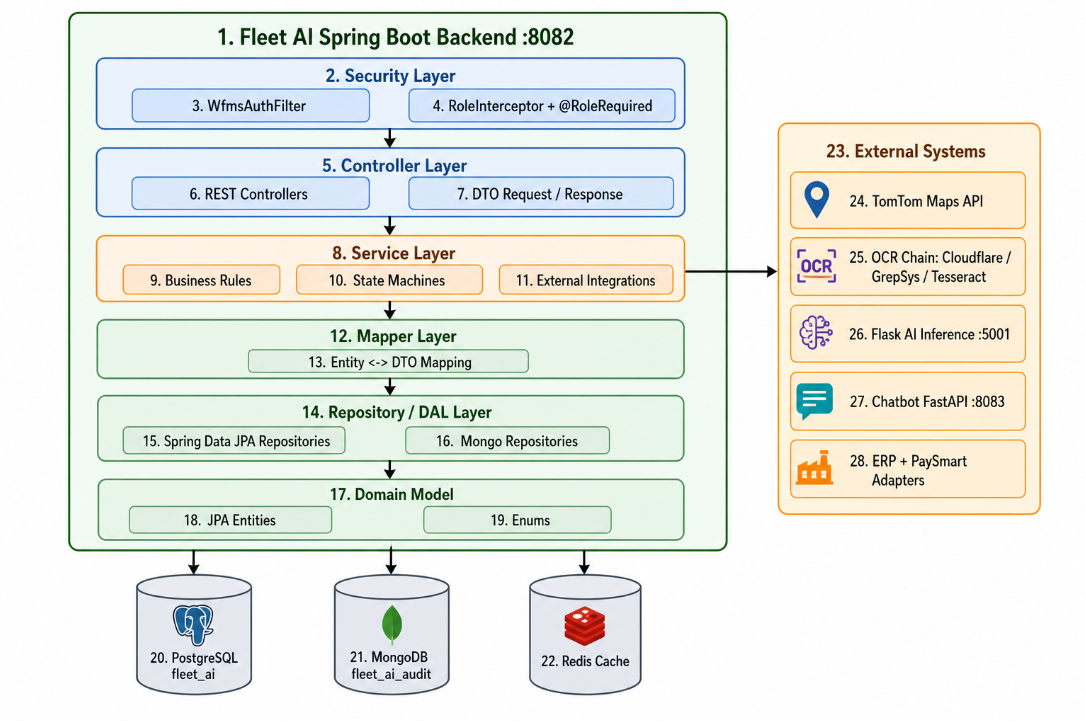
\includegraphics[width=\linewidth]{img/architecture/backend_architecture}
\caption{Architecture N-tiers en couches du back-end Fleet~AI}
\label{fig:archi-backend}
\end{figure}

\begin{itemize}
    \item[$\bullet$] \textbf{Controller :} Expose les endpoints REST, extrait le contexte WFMS et délègue aux services.
    \item[$\bullet$] \textbf{Service :} Contient la logique métier, les validations et les règles de gestion.
    \item[$\bullet$] \textbf{Repository :} Interface Spring Data JPA pour l'accès aux données relationnelles (PostgreSQL).
    \item[$\bullet$] \textbf{Entity :} Classes JPA avec héritage JOINED (FleetUser $\rightarrow$ Chauffeur, Administrateur, Manager, Planificateur).
    \item[$\bullet$] \textbf{DTO :} Objets de transfert séparés en \texttt{request/} et \texttt{response/} pour découpler l'API du modèle interne.
    \item[$\bullet$] \textbf{Mapper :} Convertit les entités JPA en DTOs et inversement.
    \item[$\bullet$] \textbf{Security :} Filtre d'authentification WFMS (\texttt{WfmsAuthFilter}) et intercepteur RBAC (\texttt{@RoleRequired}).
\end{itemize}

% ------ FRONTEND ARCHITECTURE ------
\subsection{Architecture du Front-end (Angular)}

Le front-end Angular~19 suit une \textbf{architecture modulaire} structurée en trois couches principales : \textbf{Core}, \textbf{Modules} (fonctionnalités métier) et \textbf{Shared} (composants réutilisables). Chaque module métier est découpé en sous-dossiers \texttt{data-access/} (services et modèles) et \texttt{pages/} (composants de vue).

\begin{figure}[H]
\centering
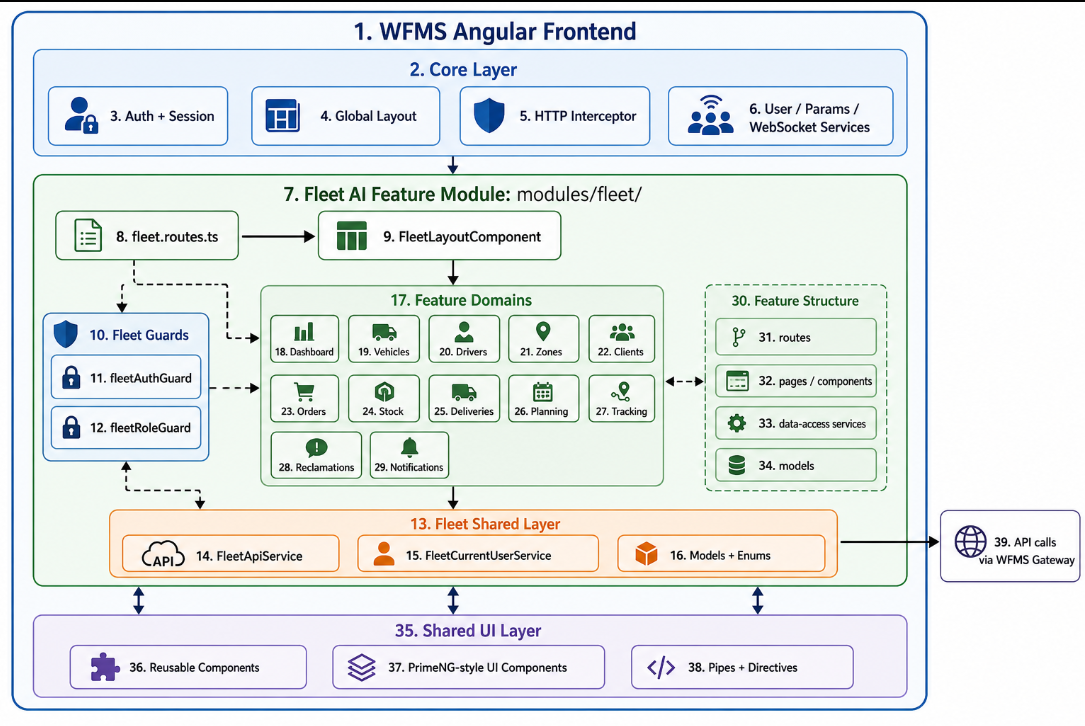
\includegraphics[width=\linewidth]{img/architecture/angular_frontend_architecture}
\caption{Architecture modulaire du front-end Angular~19}
\label{fig:archi-frontend}
\end{figure}

% ------ MOBILE ARCHITECTURE ------
\subsection{Architecture Mobile (Flutter -- MVVM)}

L'application mobile Flutter adopte le pattern \textbf{MVVM} (Model--View--ViewModel) qui sépare clairement la logique de présentation de la logique métier et de l'accès aux données.

\begin{figure}[H]
\centering
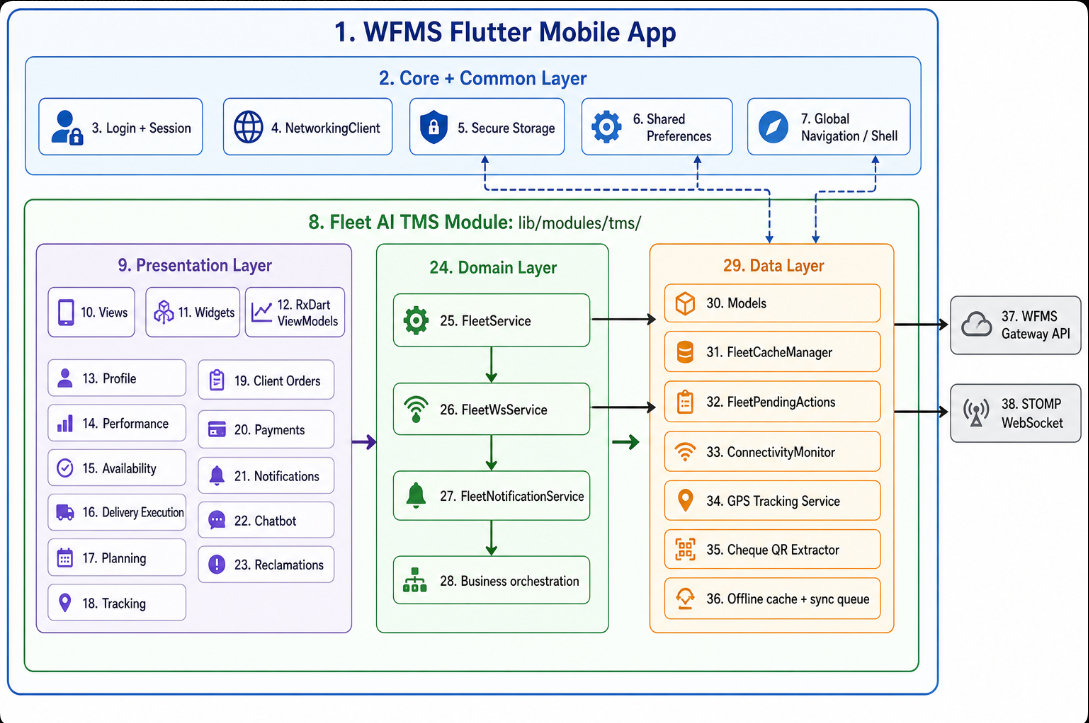
\includegraphics[width=\linewidth]{img/architecture/flutter_mvvm_architecture}
\caption{Architecture MVVM de l'application mobile Flutter}
\label{fig:archi-mobile}
\end{figure}

\begin{itemize}
    \item[$\bullet$] \textbf{View :} Les widgets Flutter affichent l'interface utilisateur et capturent les interactions de l'utilisateur (chauffeur).
    \item[$\bullet$] \textbf{ViewModel :} Gère l'état de l'application, transforme les données du modèle et notifie la vue des changements via le data binding.
    \item[$\bullet$] \textbf{Model :} Contient les entités de données, les repositories qui encapsulent l'accès aux API REST (via la passerelle WFMS) et le stockage local pour le mode hors ligne.
\end{itemize}



\section*{Conclusion}
\addcontentsline{toc}{section}{Conclusion}
La méthodologie Scrum a permis une grande flexibilité tout au long du projet. L'architecture N-Tiers associée à la passerelle WFMS offre une structure robuste pour accueillir l'ensemble des fonctionnalités que nous décrirons dans les prochains chapitres.
